\documentclass[final]{beamer}
\usepackage{lmodern}   % scalable Type1 fonts — fixes CM font size warnings with beamerposter
\mode<presentation>{\usetheme{ParisSaclay}}

% --- Override ParisSaclay theme defaults ---
% Quantum-themed background (colours + definitions inlined here)
\usetikzlibrary{backgrounds, calc}
\definecolor{bgA}{HTML}{020210}
\definecolor{bgB}{HTML}{040418}
\definecolor{bgC}{HTML}{02060E}
\definecolor{bgD}{HTML}{060214}
\definecolor{glowElectric}{HTML}{4400FF}
\definecolor{glowHot}{HTML}{FF0080}
\definecolor{glowNeon}{HTML}{00FFCC}
\definecolor{glowDeep}{HTML}{2200AA}
\definecolor{hexCbg}{HTML}{9B30FF}
\definecolor{circCbg}{HTML}{00BBFF}
\setbeamertemplate{background canvas}{%
  \begin{tikzpicture}
    \useasboundingbox (0,0) rectangle (\paperwidth,\paperheight);
    % Near-black base
    \shade[upper left=bgD, upper right=bgA,
           lower left=bgB, lower right=bgC]
      (0,0) rectangle (\paperwidth,\paperheight);
    % Vivid colour bursts
    \shade[inner color=glowElectric, outer color=bgD, opacity=0.55]
      ([xshift=8cm, yshift=-12cm]current page.north west) circle (26cm);
    \shade[inner color=glowHot, outer color=bgC, opacity=0.35]
      ([xshift=-8cm, yshift=12cm]current page.south east) circle (22cm);
    \shade[inner color=glowNeon, outer color=bgA, opacity=0.20]
      ([xshift=-6cm, yshift=0cm]current page.east) circle (18cm);
    \shade[inner color=glowDeep, outer color=bgB, opacity=0.45]
      ([xshift=6cm, yshift=6cm]current page.south west) circle (20cm);
    % Diagonal hexagons
    \begin{scope}[hexCbg, line width=3.5pt, opacity=0.45]
      \draw ([xshift=6cm, yshift=9cm]current page.south west)
        ++(15:7cm) -- ++(75:7cm) -- ++(135:7cm)
        -- ++(195:7cm) -- ++(255:7cm) -- ++(315:7cm) -- cycle;
      \draw ([xshift=-7cm, yshift=2cm]current page.east)
        ++(15:8cm) -- ++(75:8cm) -- ++(135:8cm)
        -- ++(195:8cm) -- ++(255:8cm) -- ++(315:8cm) -- cycle;
      \draw ([xshift=12cm, yshift=-12cm]current page.north west)
        ++(15:6cm) -- ++(75:6cm) -- ++(135:6cm)
        -- ++(195:6cm) -- ++(255:6cm) -- ++(315:6cm) -- cycle;
      \draw ([xshift=-12cm, yshift=-10cm]current page.north east)
        ++(15:4.5cm) -- ++(75:4.5cm) -- ++(135:4.5cm)
        -- ++(195:4.5cm) -- ++(255:4.5cm) -- ++(315:4.5cm) -- cycle;
      \draw ([xshift=-10cm, yshift=16cm]current page.south east)
        ++(15:5.5cm) -- ++(75:5.5cm) -- ++(135:5.5cm)
        -- ++(195:5.5cm) -- ++(255:5.5cm) -- ++(315:5.5cm) -- cycle;
      \draw ([xshift=4cm, yshift=4cm]current page.west)
        ++(15:5cm) -- ++(75:5cm) -- ++(135:5cm)
        -- ++(195:5cm) -- ++(255:5cm) -- ++(315:5cm) -- cycle;
    \end{scope}
    % Dashed echo hexagons
    \begin{scope}[hexCbg, line width=2pt, opacity=0.22, dashed]
      \draw ([xshift=6cm, yshift=9cm]current page.south west)
        ++(15:10cm) -- ++(75:10cm) -- ++(135:10cm)
        -- ++(195:10cm) -- ++(255:10cm) -- ++(315:10cm) -- cycle;
      \draw ([xshift=-7cm, yshift=2cm]current page.east)
        ++(15:11cm) -- ++(75:11cm) -- ++(135:11cm)
        -- ++(195:11cm) -- ++(255:11cm) -- ++(315:11cm) -- cycle;
      \draw ([xshift=12cm, yshift=-12cm]current page.north west)
        ++(15:9cm) -- ++(75:9cm) -- ++(135:9cm)
        -- ++(195:9cm) -- ++(255:9cm) -- ++(315:9cm) -- cycle;
    \end{scope}
    % Quantum circuit — bottom-right
    \begin{scope}[circCbg, opacity=0.35, line width=1.5pt,
                  shift={([xshift=-18cm, yshift=4cm]current page.south east)},
                  rotate=4]
      \foreach \yy in {0, 2, 4, 6, 8}{
        \draw (0, \yy cm) -- (18cm, \yy cm);
      }
      \fill[circCbg, opacity=0.40] (2cm, -0.6cm) rectangle (3.8cm, 0.6cm);
      \fill[circCbg, opacity=0.40] (6cm, 1.4cm) rectangle (7.8cm, 2.6cm);
      \fill[circCbg, opacity=0.40] (4cm, 3.4cm) rectangle (5.8cm, 4.6cm);
      \fill[circCbg, opacity=0.40] (10cm, 5.4cm) rectangle (11.8cm, 6.6cm);
      \fill[circCbg, opacity=0.40] (12cm, 7.4cm) rectangle (13.8cm, 8.6cm);
      \fill[circCbg, opacity=0.40] (14cm, 1.4cm) rectangle (15.8cm, 2.6cm);
      \fill[circCbg, opacity=0.40] (8cm, -0.6cm) rectangle (9.8cm, 0.6cm);
      \draw[line width=2.5pt] (5cm, 0cm) -- (5cm, 2cm);
      \fill (5cm, 0cm) circle (5pt);
      \draw (5cm, 2cm) circle (7pt);
      \draw[line width=2.5pt] (11cm, 4cm) -- (11cm, 6cm);
      \fill (11cm, 4cm) circle (5pt);
      \draw (11cm, 6cm) circle (7pt);
      \draw[line width=2.5pt] (9cm, 6cm) -- (9cm, 8cm);
      \fill (9cm, 6cm) circle (5pt);
      \draw (9cm, 8cm) circle (7pt);
      \draw[line width=2.5pt] (15cm, 4cm) -- (15cm, 6cm);
      \fill (15cm, 4cm) circle (5pt);
      \draw (15cm, 6cm) circle (7pt);
      \draw[line width=2.5pt] (3cm, 2cm) -- (3cm, 4cm);
      \fill (3cm, 2cm) circle (5pt);
      \draw (3cm, 4cm) circle (7pt);
    \end{scope}
    % Quantum circuit — top-left
    \begin{scope}[circCbg, opacity=0.25, line width=1.2pt,
                  shift={([xshift=2cm, yshift=-8cm]current page.north west)},
                  rotate=-3]
      \foreach \yy in {0, 1.8, 3.6, 5.4}{
        \draw (0, \yy cm) -- (14cm, \yy cm);
      }
      \fill[circCbg, opacity=0.35] (2cm, -0.5cm) rectangle (3.5cm, 0.5cm);
      \fill[circCbg, opacity=0.35] (5cm, 1.3cm) rectangle (6.5cm, 2.3cm);
      \fill[circCbg, opacity=0.35] (9cm, 3.1cm) rectangle (10.5cm, 4.1cm);
      \fill[circCbg, opacity=0.35] (4cm, 4.9cm) rectangle (5.5cm, 5.9cm);
      \fill[circCbg, opacity=0.35] (11cm, 1.3cm) rectangle (12.5cm, 2.3cm);
      \draw[line width=2pt] (4cm, 0cm) -- (4cm, 1.8cm);
      \fill (4cm, 0cm) circle (4pt);
      \draw (4cm, 1.8cm) circle (6pt);
      \draw[line width=2pt] (8cm, 1.8cm) -- (8cm, 3.6cm);
      \fill (8cm, 1.8cm) circle (4pt);
      \draw (8cm, 3.6cm) circle (6pt);
      \draw[line width=2pt] (7cm, 3.6cm) -- (7cm, 5.4cm);
      \fill (7cm, 3.6cm) circle (4pt);
      \draw (7cm, 5.4cm) circle (6pt);
    \end{scope}
    % Border frame
    \draw[hexCbg, line width=3.5pt, opacity=0.50]
      ([xshift=0.8cm, yshift=0.8cm]current page.south west)
      rectangle
      ([xshift=-0.8cm, yshift=-0.8cm]current page.north east);
    \draw[glowHot, line width=1.5pt, opacity=0.25]
      ([xshift=1.4cm, yshift=1.4cm]current page.south west)
      rectangle
      ([xshift=-1.4cm, yshift=-1.4cm]current page.north east);
  \end{tikzpicture}%
}
% Taller footline so the dark bar fully covers the author/institute text
\setbeamertemplate{footline}{
  \leavevmode%
  \begin{beamercolorbox}[wd=\paperwidth,ht=4ex,dp=2ex,leftskip=1.5em,rightskip=1.5em]{footline}%
    \insertauthor\hfill CentraleSup\'elec\hfill\insertdate
    \vskip1ex
  \end{beamercolorbox}%
  \begin{beamercolorbox}[wd=\paperwidth]{lower separation line foot}
    \rule{0pt}{3pt}
  \end{beamercolorbox}
}
% Replace \faSplotch bullets with standard bullets
\setbeamertemplate{itemize item}{\raisebox{0.1ex}{$\bullet$}\hskip0.2em}
\setbeamertemplate{itemize subitem}{\raisebox{0.1ex}{$\triangleright$}\hskip0.2em}
% -------------------------------------------

\usepackage[english]{babel}
\usepackage[latin1]{inputenc}
\usepackage{amsmath,amsthm,amssymb,latexsym}
\usepackage{booktabs}
\usepackage{multirow}
\usepackage{graphicx}
\usepackage{tikz}
\usetikzlibrary{positioning}

\boldmath
\usepackage[orientation=portrait,size=a1,scale=1.2]{beamerposter}

\title{\huge RL-Based quantum circuit routing:\\ Optimizing qubit mapping via Deep RL}
\author{Elora Drouilhet \and Ali El Dor}
\institute[]{CentraleSup\'elec}

\begin{document}
\begin{frame}[fragile]{}

\begin{columns}[t]

% ============================================================
%  LEFT COLUMN
% ============================================================
\begin{column}{.46\textwidth}

\begin{alertblock}{Motivation \& problem}
\normalsize
Quantum hardware has limited connectivity: two-qubit gates can only run on \textbf{neighbouring} qubits.
When qubits are far apart, the compiler must insert \textbf{SWAP gates} (each = 3~CNOTs), increasing depth and noise.
The qubit routing problem is \textbf{NP-hard}~[2].

\smallskip
\textbf{Goal:} learn a policy that inserts SWAPs to route all gates while \textbf{minimising overhead}.\\
\textbf{Question:} Can a CNN-based RL agent \textbf{beat SABRE}, the industry-standard router?
\end{alertblock}

\vspace{0.05cm}

\begin{block}{Environment}
\textbf{State} -- padded $27\!\times\!27\!\times\!5$ tensor:
Ch\,0 adjacency, Ch\,1 mapping, Ch\,2 depth-decayed gate demand ($\gamma{=}0.5$),
Ch\,3 front-layer distance, Ch\,4 stagnation signal.
Channels 3--4 fixed Q-value collapse from the original 3-channel design.

\smallskip
\textbf{Action:} choose one hardware edge $\Rightarrow$ SWAP.
After each SWAP, all newly routable front-layer gates are \textbf{auto-executed}.

\smallskip
\textbf{Reward:}
$r = \underbrace{g \cdot n_{\text{gates}}}_{\text{gate}} + \underbrace{\alpha\,\Delta d}_{\text{distance}} \underbrace{{}- c_{\text{step}}}_{\text{step}} \underbrace{{}- c_{\text{backtrack}}}_{\text{reverse}} \underbrace{{}- c_{\text{repeat}}}_{\text{same-edge}} \underbrace{{}- c_{\text{stall}}}_{\text{no-progress}} + \underbrace{r_{\text{done}}}_{\text{terminal}}$\\
{\small Per-step: gates executed ($+1$), distance shaping ($\alpha{=}0.1$), step cost ($-0.05$), reverse-SWAP ($-0.2$), same-edge ($-0.2{\times}\text{streak}$), no-progress ($-0.03{\times}\text{streak}$). Terminal: end ($+15$) / timeout ($-8$).}
\end{block}

\vspace{0.05cm}

\begin{block}{Agents}
\begin{itemize}
  \item \textbf{PPO -- Symmetry-aware CNN actor-critic}\\
    {\small 3-layer CNN backbone; symmetric pairwise score map; 3-stage curriculum
    (\texttt{linear\_5} $\to$ \texttt{grid\_3x3} $\to$ \texttt{heavy\_hex\_19});
    anti-collapse via progressive logit penalty + no-progress truncation}
  \item \textbf{D3QN + PER -- value-based agent}\\
    {\small Dueling Double DQN + prioritized replay (${\sim}6$M params);
    Conv $5{\to}32{\to}64{\to}32$, dueling V/A streams;
    soft target updates ($\tau{=}0.005$/500 steps); $\varepsilon$: $1.0 \to 0.02$}
\end{itemize}
\end{block}

\vspace{0.05cm}

\begin{block}{Architecture}
\begin{center}
  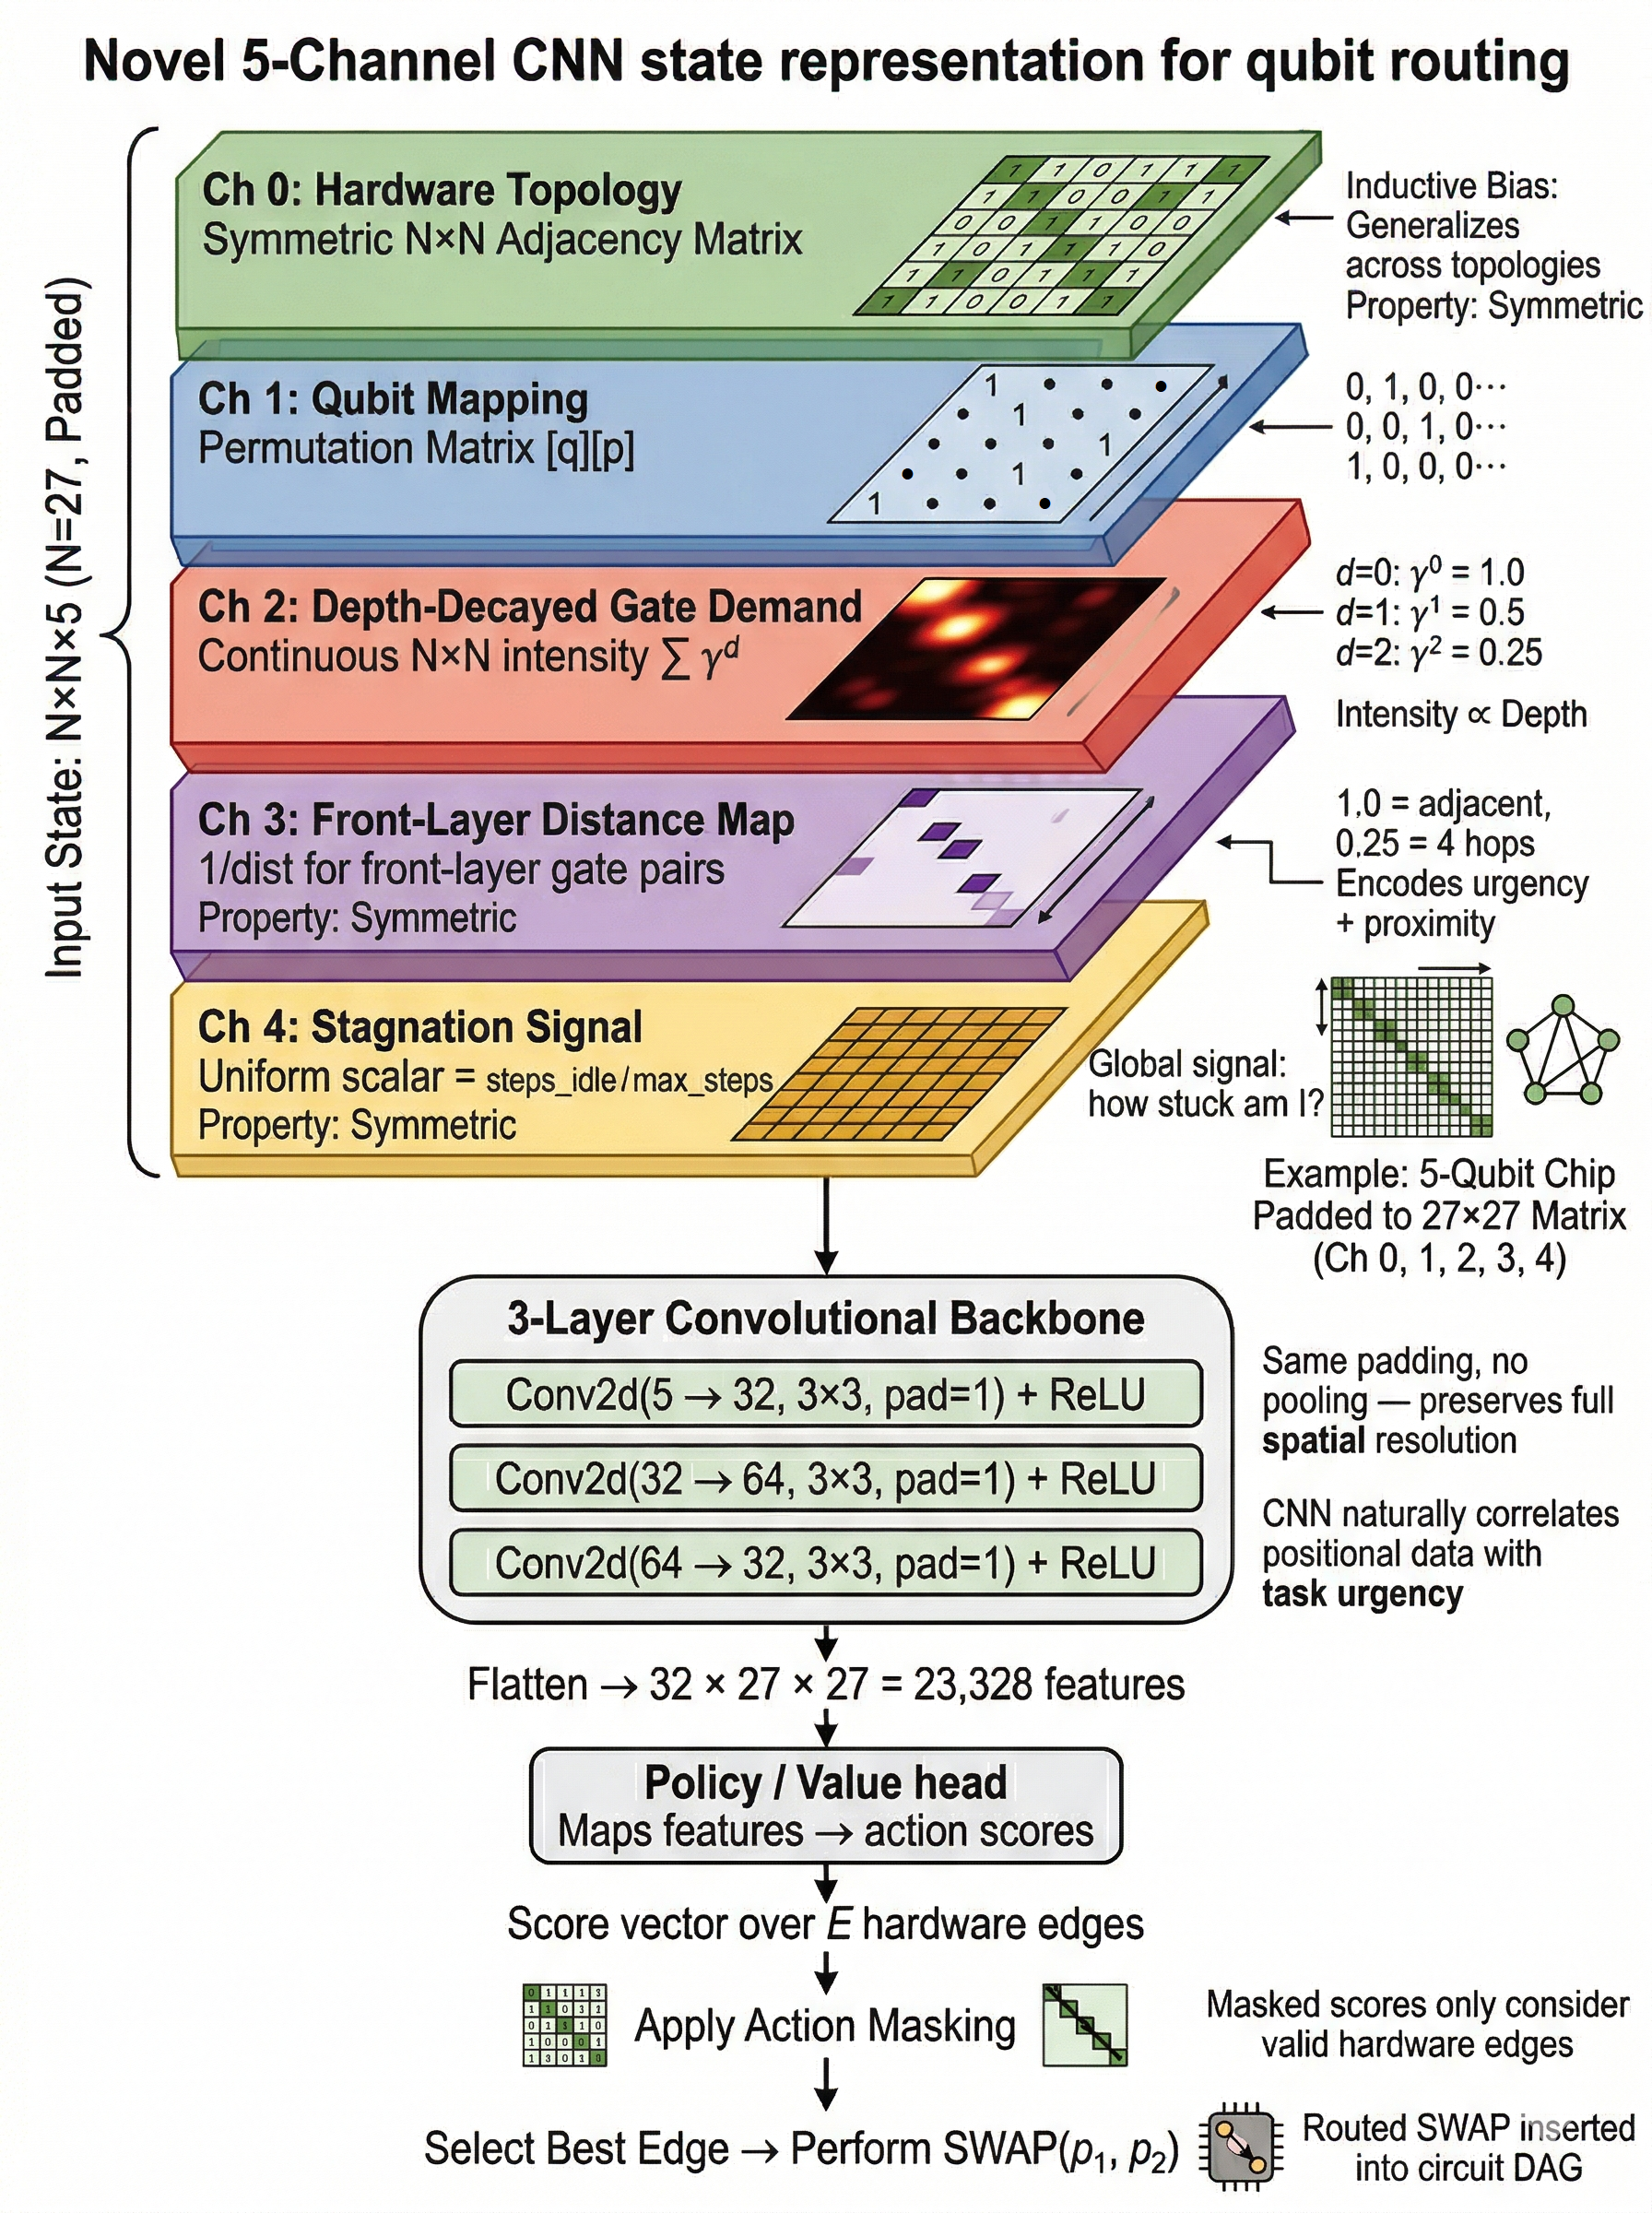
\includegraphics[width=1\textwidth]{Architecture.png}
\end{center}
\end{block}

\vspace{0.05cm}

\begin{block}{Hardware topologies \& experimental setup}
{\small
\begin{itemize}
  \item Random circuits on-the-fly (training); QASMBench (eval)
  \item Baseline: \textbf{SABRE}~[1] -- state-of-the-art classical router
  \item Metric: \textbf{SWAP ratio} = agent / SABRE ($<1.0$ = beats SABRE)
  \item 23 experiments across 5 versions, 60--80k episodes each
\end{itemize}
}
\vspace{0.05cm}
\begin{center}
\begin{tikzpicture}[
    q/.style={circle, draw=blue!70!black, fill=blue!15, inner sep=0pt,
              minimum size=9pt, line width=0.6pt},
    lbl/.style={font=\small, blue!70!black}
  ]
  % -- linear_5 --
  \foreach \i in {0,...,4}{ \node[q] (l\i) at (\i*0.7, 0) {}; }
  \draw (l0)--(l1)--(l2)--(l3)--(l4);
  \node[lbl] at (1.4,-0.45) {\texttt{linear\_5}};
  % -- grid_3x3 --
  \foreach \c in {0,1,2}{
    \foreach \r in {0,1,2}{
      \node[q] (g\r\c) at ({4.2+\c*0.7},{-\r*0.7}) {};
    }
  }
  \foreach \r in {0,1,2}{ \draw (g\r0)--(g\r1)--(g\r2); }
  \foreach \c in {0,1,2}{ \draw (g0\c)--(g1\c)--(g2\c); }
  \node[lbl] at (4.9,-1.90) {\texttt{grid\_3x3}};
  % -- heavy_hex_19 --
  \foreach \i in {0,...,4}{ \node[q] (h0\i) at ({9.0+\i*0.6}, 0) {}; }
  \foreach \i in {0,...,3}{ \node[q] (h1\i) at ({9.3+\i*0.6}, -0.5) {}; }
  \foreach \i in {0,...,4}{ \node[q] (h2\i) at ({9.0+\i*0.6}, -1.0) {}; }
  \foreach \i in {0,...,3}{ \node[q] (h3\i) at ({9.3+\i*0.6}, -1.5) {}; }
  \node[q] (h40) at (9.9, -2.0) {};
  \foreach \i in {0,...,3}{ \pgfmathtruncatemacro{\j}{\i+1} \draw (h0\i)--(h0\j); }
  \foreach \i in {0,...,3}{ \pgfmathtruncatemacro{\j}{\i+1} \draw (h2\i)--(h2\j); }
  \draw (h01)--(h10); \draw (h02)--(h11); \draw (h03)--(h12); \draw (h04)--(h13);
  \draw (h10)--(h21); \draw (h11)--(h22); \draw (h12)--(h23); \draw (h13)--(h24);
  \draw (h21)--(h30); \draw (h22)--(h31); \draw (h23)--(h32); \draw (h24)--(h33);
  \draw (h31)--(h40);
  \node[lbl] at (10.2,-2.5) {\texttt{heavy\_hex\_19}};
\end{tikzpicture}
\end{center}
\end{block}

\end{column}

% ============================================================
%  RIGHT COLUMN
% ============================================================
\begin{column}{.46\textwidth}

\begin{block}{Results: D3QN}
\begin{center}
{\small
\begin{tabular}{lcccr}
\toprule
\textbf{Topology} & \textbf{Ratio} & \textbf{Win \%} & \textbf{Compl.} & \textbf{Config} \\
\midrule
\multicolumn{5}{l}{\textit{Single-topology}} \\
\texttt{heavy\_hex\_19} & \textbf{0.991} & 94 & 100\% & 80k ep. \\
\texttt{heavy\_hex\_19} & \textbf{0.994} & -- & 100\% & 60k ep., curriculum \\
\midrule
\multicolumn{5}{l}{\textit{Multi-topology (single agent, all 3 topologies)}} \\
\texttt{linear\_5}      & \textbf{0.890} & -- & 100\% & \multirow{4}{*}{60k ep., bignet} \\
\texttt{grid\_3x3}      & 1.008          & -- & 100\% & \\
\texttt{heavy\_hex\_19} & 1.107          & -- & 100\% & \\
\textbf{Overall}        & \textbf{0.999} & -- & 100\% & \\
\bottomrule
\end{tabular}
}
\end{center}
\vspace{-0.1cm}
{\small \textbf{Best:} ratio \textbf{0.991} on \texttt{heavy\_hex\_19} (183.3 vs 185.3~SWAPs).
Curriculum variant reaches 0.994 in 25\% less training time.
A single multi-topology agent matches SABRE overall (0.999) and \textbf{beats it by 11\%} on \texttt{linear\_5}.}

\vspace{0.05cm}
\begin{center}
  
\includegraphics[width=1\textwidth]{eval_comparison_run019}
\end{center}
\vspace{-0.2cm}
{\small D3QN (blue) vs SABRE (orange): per-circuit SWAP counts at best checkpoint. The agent wins or matches on the majority of 50 random depth-20 circuits on \texttt{heavy\_hex\_19}.}
\end{block}

\vspace{0.05cm}

\begin{block}{Results: PPO}
\begin{center}
{\small
\begin{tabular}{lcccr}
\toprule
\textbf{Topology} & \textbf{Ratio} & \textbf{Win \%} & \textbf{Compl.} & \textbf{Config} \\
\midrule
\multicolumn{5}{l}{\textit{Single-topology}} \\
\texttt{linear\_5}      & \textbf{0.871} & 94 & 100\% & 2M steps \\
\texttt{grid\_3x3}      & 1.096          & 38 & 100\% & 10M steps, LR anneal \\
\texttt{heavy\_hex\_19} & \multicolumn{4}{c}{\textit{in progress}} \\
\bottomrule
\end{tabular}
}
\end{center}
\vspace{-0.1cm}
{\small \textbf{Best:} PPO \textbf{beats SABRE by 12.9\%} on \texttt{linear\_5} (14.1 vs 16.2~SWAPs).
On \texttt{grid\_3x3}, LR annealing ($3{\times}10^{-4}{\to}3{\times}10^{-5}$) eliminated late-training regression.
Key contribution: \textbf{anti-collapse engineering} -- logit penalties, progressive same-edge penalty, and dynamic truncation enabled stable PPO training across 9 design iterations.}
\end{block}

\vspace{0.05cm}

\begin{block}{D3QN training dashboard}
\begin{center}
  
\includegraphics[width=0.95\textwidth]{training_curves_run019}
\end{center}
\vspace{-0.3cm}
{\small \textbf{Top row:} episode reward convergence; SWAP count (blue) crossing below the SABRE baseline (orange); completion rate jumping 0\%$\to$100\% during the phase transition at ${\sim}$ep\,8k.
\textbf{Bottom row:} Huber loss stabilisation; $\varepsilon$-greedy decay; mean Q-value and TD error evolution.}
\end{block}

\vspace{0.05cm}

\begin{block}{Key findings \& ablations}
{\small
\begin{itemize}
  \item \textbf{5-ch state solved Q-collapse}: Ch\,3--4 eliminated degenerate policies in both agents
  \item \textbf{PPO vs D3QN}: PPO best on \texttt{linear\_5} (0.871 vs 0.890); D3QN best on harder topologies -- PER focuses on difficult transitions, an advantage on-policy methods lack
  \item \textbf{LR annealing prevents regression}: PPO \texttt{grid\_3x3} improved from 1.24 to 1.096 with decay $3{\times}10^{-4}{\to}3{\times}10^{-5}$
  \item \textbf{More episodes $\gg$ bigger network}: [32,64,32] outperforms [64,128,64] (ratio 1.014 vs 1.160)
  \item \textbf{Reward sensitivity}: doubling gate reward degraded D3QN ratio to 1.377
\end{itemize}
}
\end{block}

\vspace{0.05cm}

\begin{block}{Conclusion \& future work}
{\small
\begin{itemize}
  \item \textbf{Both agents beat SABRE}: D3QN on \texttt{heavy\_hex\_19} (0.991), PPO on \texttt{linear\_5} (0.871) -- single forward pass, no search
  \item \textbf{Anti-collapse engineering} (logit penalties, progressive penalties, truncation) is essential for stable PPO on combinatorial action spaces
  \item \textbf{Future:} PPO on \texttt{heavy\_hex}, larger topologies, hybrid RL+MCTS
\end{itemize}
}
\end{block}

\vspace{0.05cm}

\begin{exampleblock}{References}
\scriptsize
[1]~Li et al., \textit{Qubit Mapping for NISQ}, ASPLOS'19.\;
[2]~Siraichi et al., \textit{Qubit Allocation}, CGO'18.\;
[3]~Schulman et al., \textit{PPO}, 2017.\;
[4]~Schaul et al., \textit{PER}, ICLR'16.\;
[5]~Wang et al., \textit{Dueling DQN}, ICML'16.
\end{exampleblock}

\end{column}
\end{columns}

\end{frame}
\end{document}
